% PhantomShield Final Year Project Report
% LaTeX version generated for SPECTER-main

\documentclass[conference]{IEEEtran}
\usepackage[utf8]{inputenc}
\usepackage{graphicx}
\usepackage{booktabs}
\usepackage{hyperref}
\usepackage{enumitem}
\usepackage{caption}
\usepackage{geometry}
\geometry{margin=0.75in}

\begin{document}

\title{PhantomShield: AI-Enabled Phishing Detection and Explanation System}

\author{\IEEEauthorblockN{[Author Name]}
\IEEEauthorblockA{Department of [Department Name] \\
[University Name] \\
Email: [email@example.com]}}

\maketitle

\begin{abstract}
PhantomShield is an AI-enabled phishing detection system that evaluates suspicious URLs, email bodies, and SMS messages through hybrid analysis. The system combines a FastAPI backend and React frontend with an ensemble of Random Forest and XGBoost classifiers. It uses 28 engineered security features, visual threat scoring, attack-type classification, AI-generated explanations, and contextual educational tips. The completed prototype illustrates how hybrid feature engineering and ensemble learning can provide robust phishing detection while helping users understand and learn from suspicious content.
\end{abstract}

\begin{IEEEkeywords}
phishing detection, ensemble learning, explainable security, FastAPI, React, homograph detection, URL analysis, cybersecurity education.
\end{IEEEkeywords}

\section{Introduction}
Phishing attacks remain one of the most widespread and damaging cybersecurity threats. Attackers create deceptive URLs, emails, and SMS messages designed to convince users to share passwords, financial details, or other sensitive information. Traditional protection methods such as blocklists and signature-based filters are not sufficient because phishing campaigns frequently employ new and customized domains.

PhantomShield addresses this gap by providing a hybrid detection system that evaluates suspicious content through structured feature analysis, machine learning, and clear explanation. The system supports URL, email, and SMS scanning with an emphasis on real-time feedback and user education.

\section{Motivation and Objectives}
The motivation for PhantomShield is driven by the following factors:
\begin{itemize}[itemsep=0pt,topsep=0pt]
    \item Phishing incidents are growing across web and mobile communication channels.
    \item Attackers increasingly use brand impersonation, homograph domains, and urgency language.
    \item Users often dismiss simple warnings without understanding the reason.
    \item A combined machine learning and rule-based approach can both detect threats and teach safer behavior.
\end{itemize}

The main objectives of PhantomShield are:
\begin{enumerate}[itemsep=0pt,topsep=0pt]
    \item Build a multi-channel phishing detection engine supporting URL, email, and SMS inputs.
    \item Design a feature engineering pipeline for URL and domain risk signals.
    \item Implement a weighted ensemble of Random Forest and XGBoost classifiers.
    \item Develop a user-friendly React frontend for scanning and results visualization.
    \item Provide explainable results and educational tips for suspicious detections.
    \item Persist scan history and user security metrics in a database.
    \item Validate detection performance through realistic test cases.
    \item Integrate recent research findings from the project literature.
\end{enumerate}

\section{Literature Survey}
The literature survey draws from the papers available in the \texttt{research paper set} folder, including the two papers in \texttt{research paper set/published paper}. The survey identifies detection patterns, model strategies, and user-centric explainability approaches relevant to PhantomShield.

Key contributions from the literature include:
\begin{itemize}[itemsep=0pt,topsep=0pt]
    \item Hybrid URL feature selection for phishing detection.
    \item Ensemble and boosting model architectures.
    \item Homograph and brand impersonation defense techniques.
    \item Explainable outputs and user education in security tools.
    \item Evaluation methodologies for phishing classification.
\end{itemize}

\section{Problem Definition}
Phishing attacks are difficult to detect using static rules alone. Users need an intelligent system that can identify suspicious URLs, email content, and SMS messages, compute a clear threat score, classify attack types, provide actionable explanation, and educate users on risk prevention.

This project addresses the need for a hybrid phishing detection system capable of real-time scanning and explainable reporting for multiple communication channels.

\section{Software Requirement Specification}
\subsection{Functional Requirements}
\begin{itemize}[itemsep=0pt,topsep=0pt]
    \item Accept input URLs and return a phishing threat score.
    \item Support email and SMS scans by extracting embedded URLs or analyzing text.
    \item Extract engineered features from URLs and domains.
    \item Compute a weighted ensemble prediction using Random Forest and XGBoost.
    \item Categorize threat levels as safe, suspicious, dangerous, or critical.
    \item Deliver explanations for suspicious results.
    \item Provide educational tips based on detected attack patterns.
    \item Persist scan history and security metrics in a database for returning users.
    \item Present results in a responsive React frontend.
    \item Retain recent scans locally if the backend is unavailable.
    \item Display analytics and weak spot metrics on a dashboard.
\end{itemize}

\subsection{Non-Functional Requirements}
\begin{itemize}[itemsep=0pt,topsep=0pt]
    \item Respond to scan requests within a few seconds.
    \item Be accessible through a web-based interface.
    \item Be scalable to support additional scan routes and model updates.
    \item Use secure communication policies for API requests.
    \item Be maintainable and modular.
    \item Log errors and warnings for troubleshooting.
    \item Support responsive UI behavior during scans.
    \item Cache recent scans in local storage when possible.
\end{itemize}

\subsection{System Constraints}
A working PhantomShield system requires Python 3.10+ with FastAPI, React and Vite for the frontend, and PostgreSQL-compatible storage. Model artifacts need to be available locally, and the system requires environment variables for database connectivity and optional Gemini explanation APIs.

\section{Proposed System Architecture}
The system comprises three core layers:
\begin{itemize}[itemsep=0pt,topsep=0pt]
    \item Frontend: React application for user interactions and visualization.
    \item Backend: FastAPI service for scanning, classification, explanation, and persistence.
    \item Database: PostgreSQL-compatible storage for scan records and user analytics.
\end{itemize}

The backend also integrates an explanation service and education engine. The architecture separates user interface concerns from the analytics and persistence layers.

\begin{figure}[ht]
    \centering
    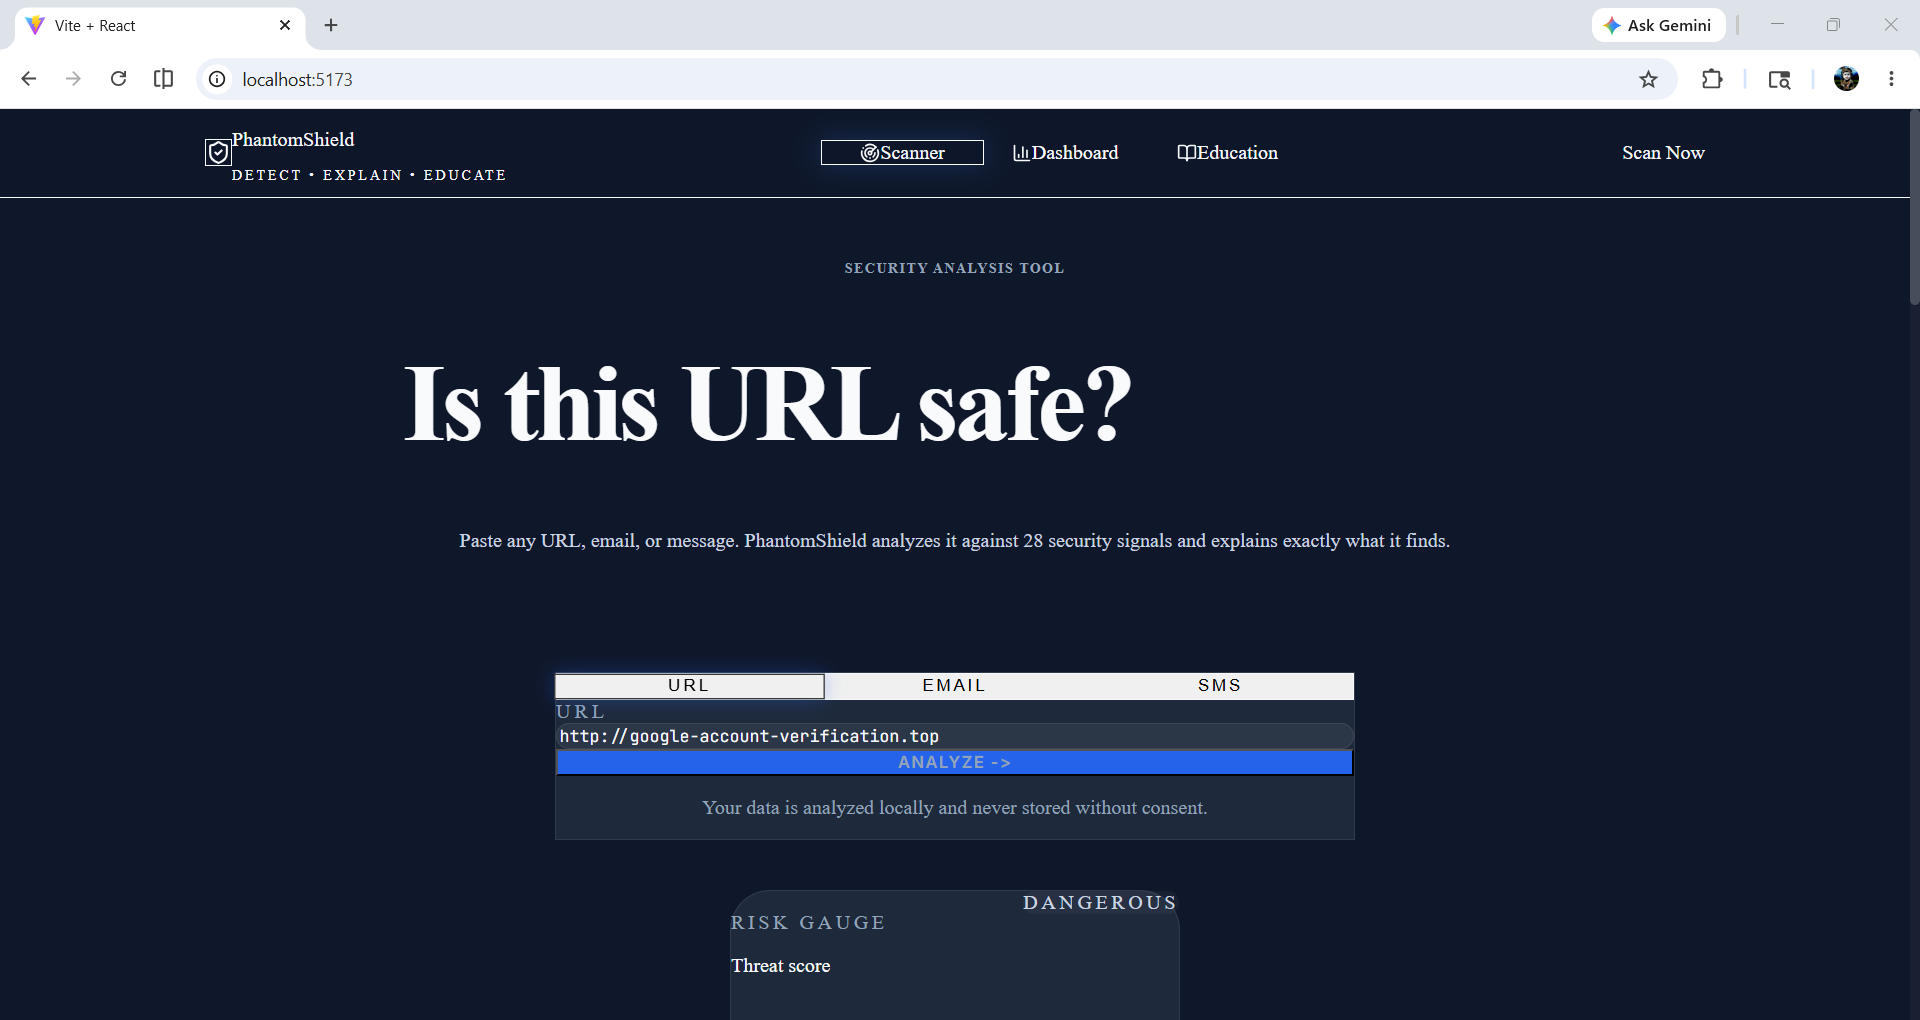
\includegraphics[width=0.98\linewidth]{screenshots/url.png}
    \caption{PhantomShield system architecture overview showing frontend, backend, and database interaction.}
    \label{fig:architecture}
\end{figure}

\section{High Level Design}
\subsection{Data Flow Diagram}
The core data flow is:
\begin{quote}
User input $\rightarrow$ Frontend scan request $\rightarrow$ Backend scan service $\rightarrow$ Feature extractor $\rightarrow$ ML predictor $\rightarrow$ Response generator $\rightarrow$ Frontend.
\end{quote}

\subsection{Component Diagram}
The system includes these major software components:
\begin{itemize}[itemsep=0pt,topsep=0pt]
    \item `ScanInput.jsx`, `ScanResult.jsx`, and `Dashboard.jsx` on the frontend.
    \item `backend/routers/scan.py`, `backend/services/url_scanner.py`, `backend/ml/predictor.py`, and `backend/services/supabase_service.py` on the backend.
    \item Explanation, education, and persistence modules.
\end{itemize}

\begin{figure}[ht]
    \centering
    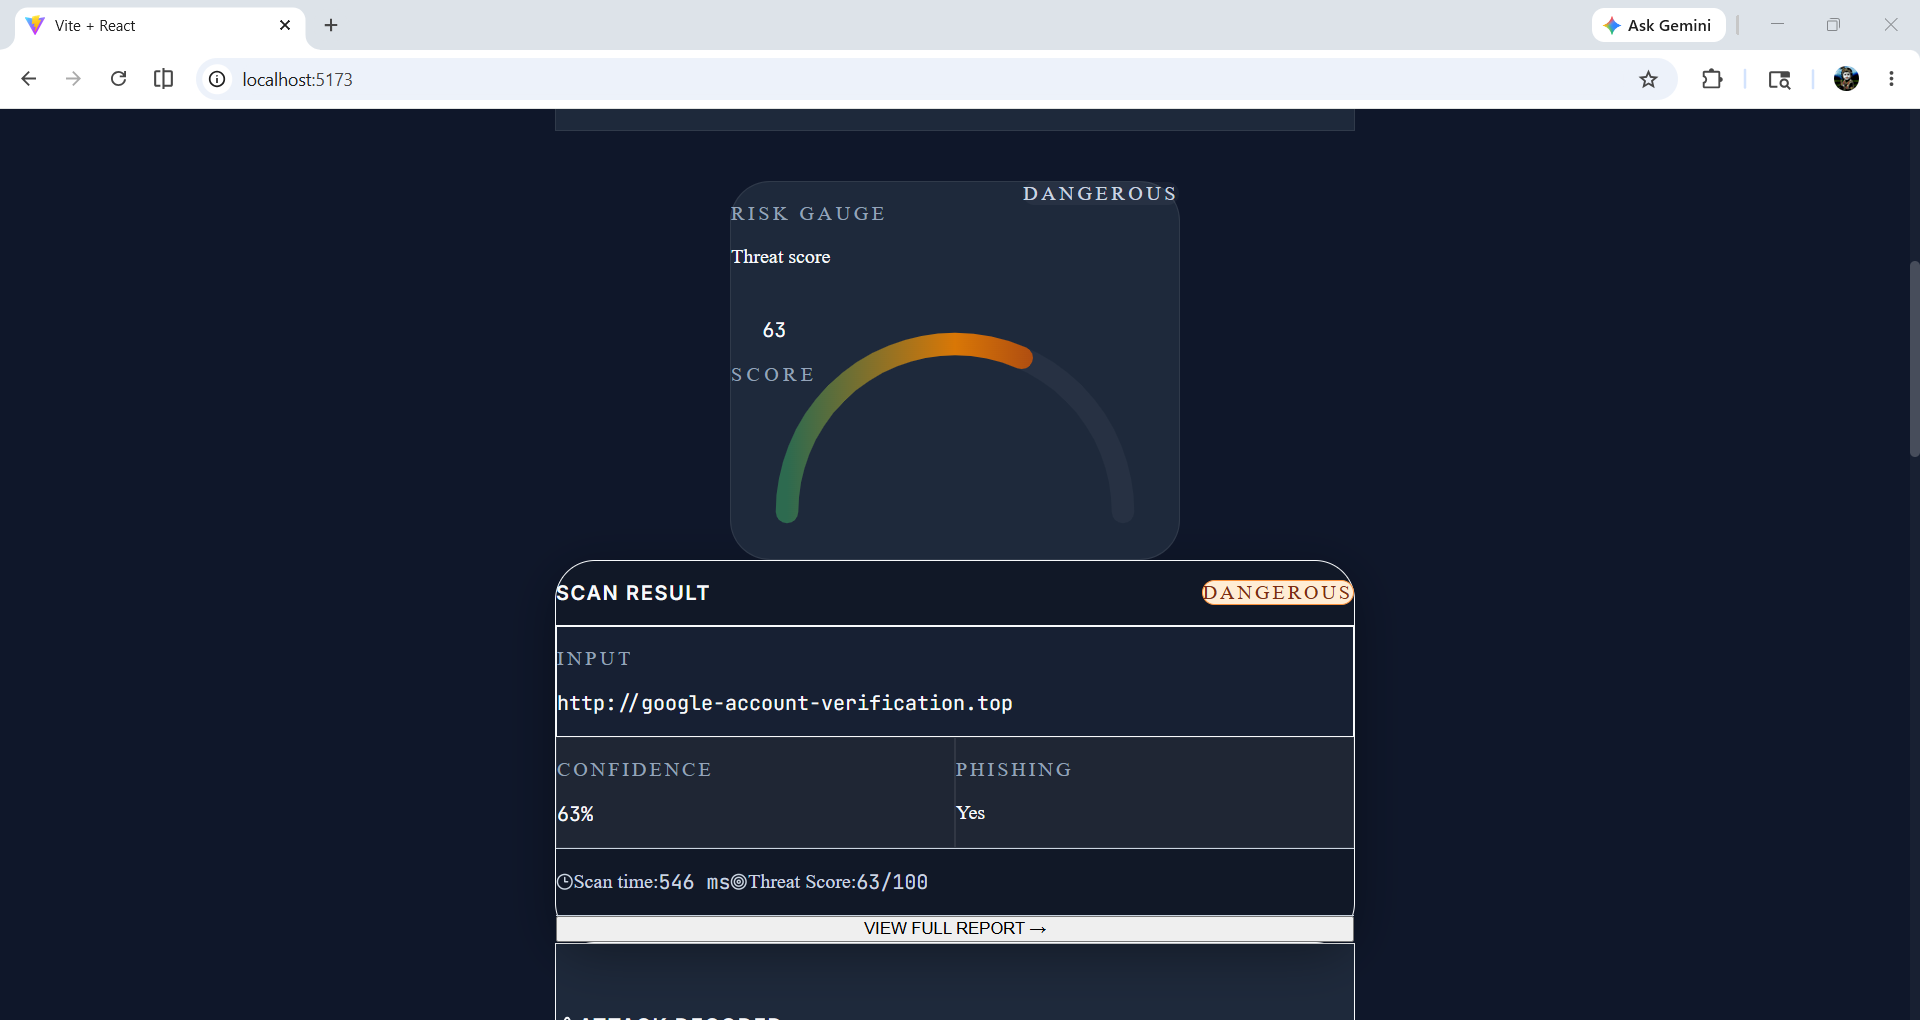
\includegraphics[width=0.98\linewidth]{screenshots/url1.png}
    \caption{URL scan workflow from input to explanation and persistence.}
    \label{fig:workflow}
\end{figure}

\subsection{ER Diagram}
The primary entities are `UserProfile` and `ScanResult`. User profiles store aggregate security metrics, while scan results store individual scan metadata and classification.

\section{System Implementation and Code Documentation}
\subsection{Algorithm and Methodology}
The scan pipeline is implemented in discrete stages:
\begin{enumerate}[itemsep=0pt,topsep=0pt]
    \item Normalize and validate the external input.
    \item Extract security features using `backend/ml/feature_extractor.py`.
    \item Load models and scale the feature vector in `backend/ml/predictor.py`.
    \item Compute the ensemble score and convert it to a threat level.
    \item Determine attack type labels.
    \item Generate explanation and education outputs.
    \item Optionally persist the result in the database.
\end{enumerate}

\subsection{Feature Extraction}
The feature extractor computes 28 signals across six categories:
\begin{itemize}[itemsep=0pt,topsep=0pt]
    \item Domain-level metrics: domain length, subdomain count, IP usage, suspicious TLD, brand impersonation, domain age.
    \item URL structure metrics: URL length, `@` symbol, double slash, special character usage, digit ratio, hyphen count, dot count, query parameters.
    \item Homograph signals: Unicode or look-alike characters and homograph count.
    \item SSL signals: HTTPS usage, SSL validity, certificate age score.
    \item Keyword indicators: login, secure, verify, update, urgency.
    \item Path and redirect signals: path depth, redirect markers, subdomain depth.
\end{itemize}
These features enable the model to distinguish legitimate and malicious URL patterns.

\subsection{Prediction and Heuristic Layer}
The backend loads Random Forest and XGBoost models and computes a weighted ensemble probability. The ensemble formula is approximately 0.45 * RF + 0.55 * XGBoost. A heuristic layer adjusts the score when strong phishing patterns are present, improving sensitivity to targeted attacks.

\subsection{Attack Type Classification}
Attack type labels are assigned based on detected patterns:
\begin{itemize}[itemsep=0pt,topsep=0pt]
    \item Homograph attacks for look-alike characters.
    \item Brand impersonation for trusted-brand text in domain names.
    \item Credential harvesting for raw IP or suspicious host patterns.
    \item Urgency manipulation for phishing language.
    \item Fake SSL for invalid certificates combined with security keywords.
    \item Typosquatting for suspicious mimic domains.
\end{itemize}

\subsection{Explanation and Education}
`backend/services/explainer_service.py` builds explanation bundles that summarize suspicious elements, their risk reasons, and recommended user actions. `backend/services/education_service.py` returns educational tips matched to the detected attack type.

\subsection{Persistence and Dashboard}
The database persistence layer stores scan records and user profile metrics. The dashboard aggregates this data for trends, weak spot analysis, and security score reporting.

\section{Test Cases}
\begin{table}[ht]
\centering
\caption{Test Case Summary}
\label{tab:testcases}
\begin{tabular}{@{}lllll@{}}
\toprule
TC ID & Description & Input & Expected Result & Status \\
\midrule
TC-01 & Safe URL scan & https://example.com & Safe score & Pass \\
TC-02 & Brand spoof & http://paypa1-secure.com/login & Suspicious & Pass \\
TC-03 & IP URL scan & http://192.168.1.1/verify & High threat & Pass \\
TC-04 & Email phishing & body with malicious URL & Suspicious & Pass \\
TC-05 & SMS urgency & urgent phishing message & Suspicious & Pass \\
TC-06 & DB persistence & valid user id & Stored result & Pass \\
TC-07 & UI navigation & all pages & Responsive load & Pass \\
TC-08 & Invalid input & blank submissions & Validation shown & Pass \\
TC-09 & Local fallback & backend disconnect & Cache visible & Pass \\
TC-10 & Model loading & missing files & Graceful warning & Pass \\
\bottomrule
\end{tabular}
\end{table}

Detailed test cases were executed to ensure functional correctness, UI robustness, and persistence behavior.

\section{GUI and Experimental Results}
The React frontend includes the following visible modules:
\begin{itemize}[itemsep=0pt,topsep=0pt]
    \item Scanner landing page.
    \item URL scan input and result panel.
    \item Email and SMS input tabs.
    \item Threat meter and explanation cards.
    \item Education library and dashboard analysis pages.
\end{itemize}

The screenshots below illustrate the working GUI and experimental results.

\begin{figure}[ht]
    \centering
    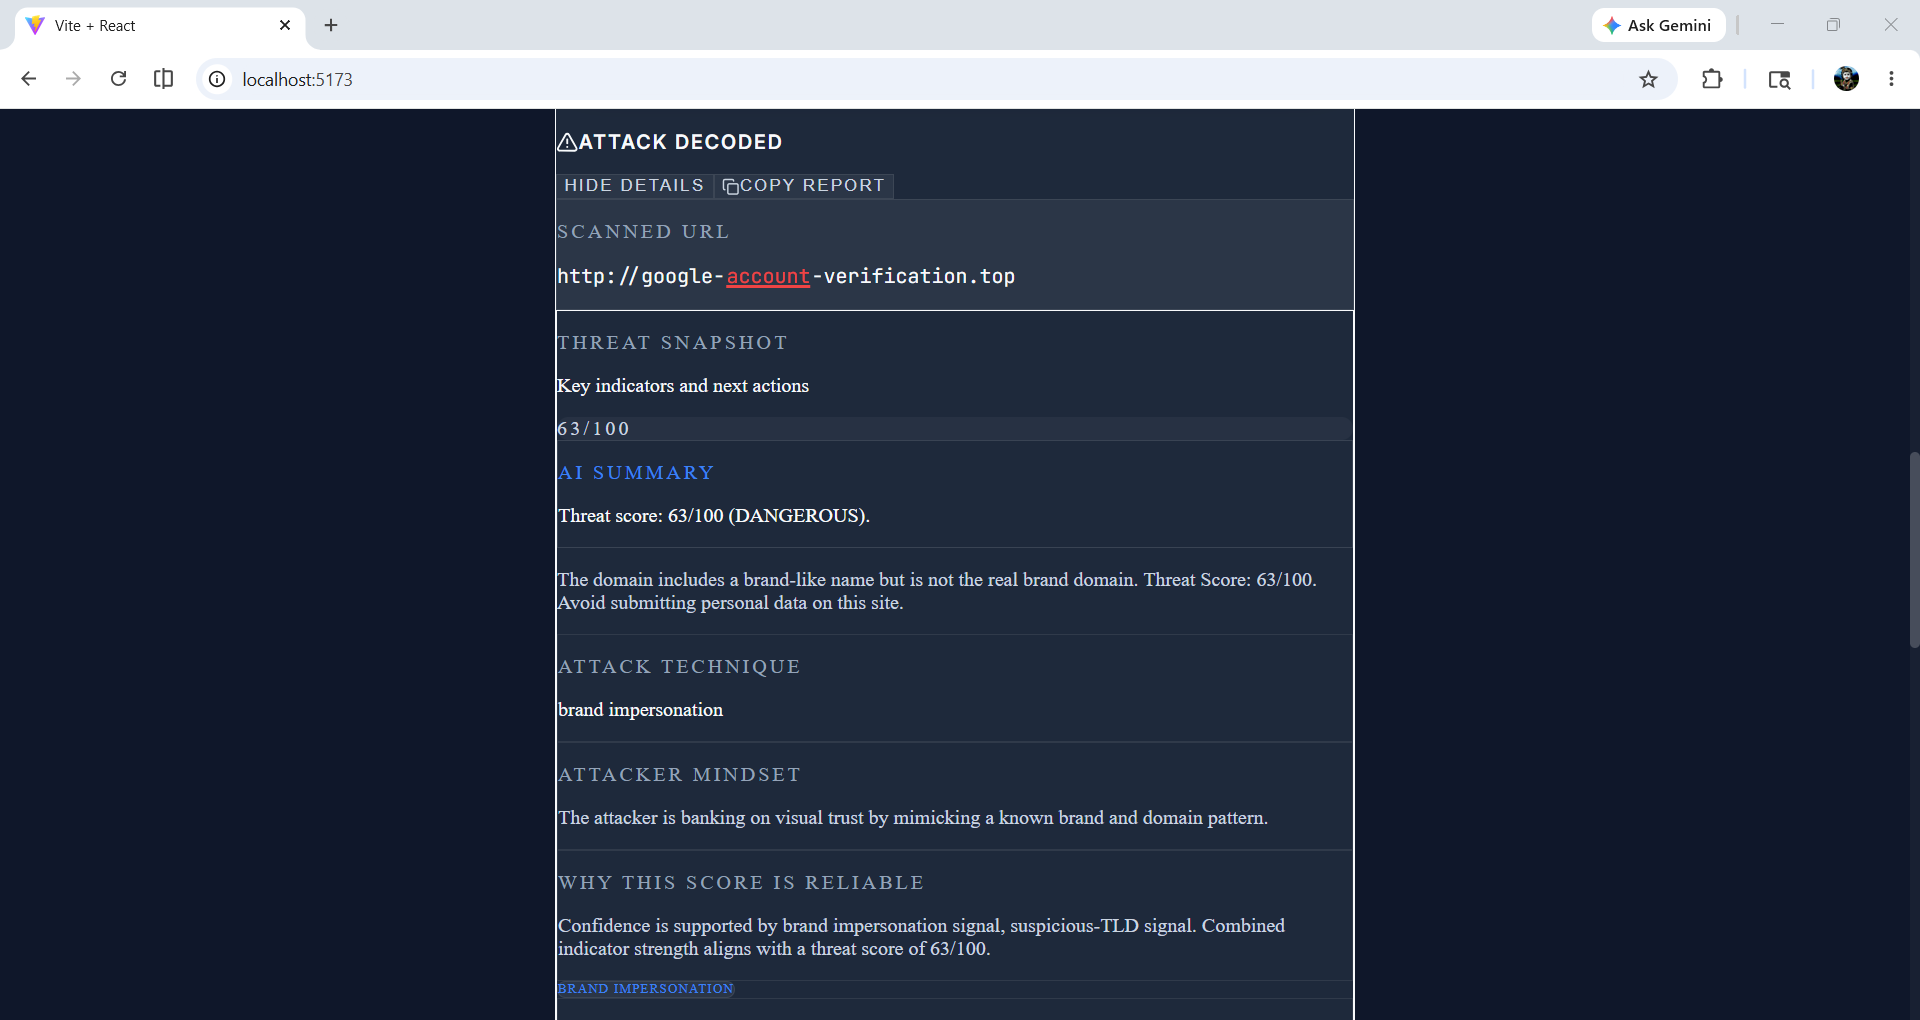
\includegraphics[width=0.98\linewidth]{screenshots/url2.png}
    \caption{Suspicious URL scan result showing threat score, verdict, explanation, and relevant security advice.}
    \label{fig:urlresult}
\end{figure}

\begin{figure}[ht]
    \centering
    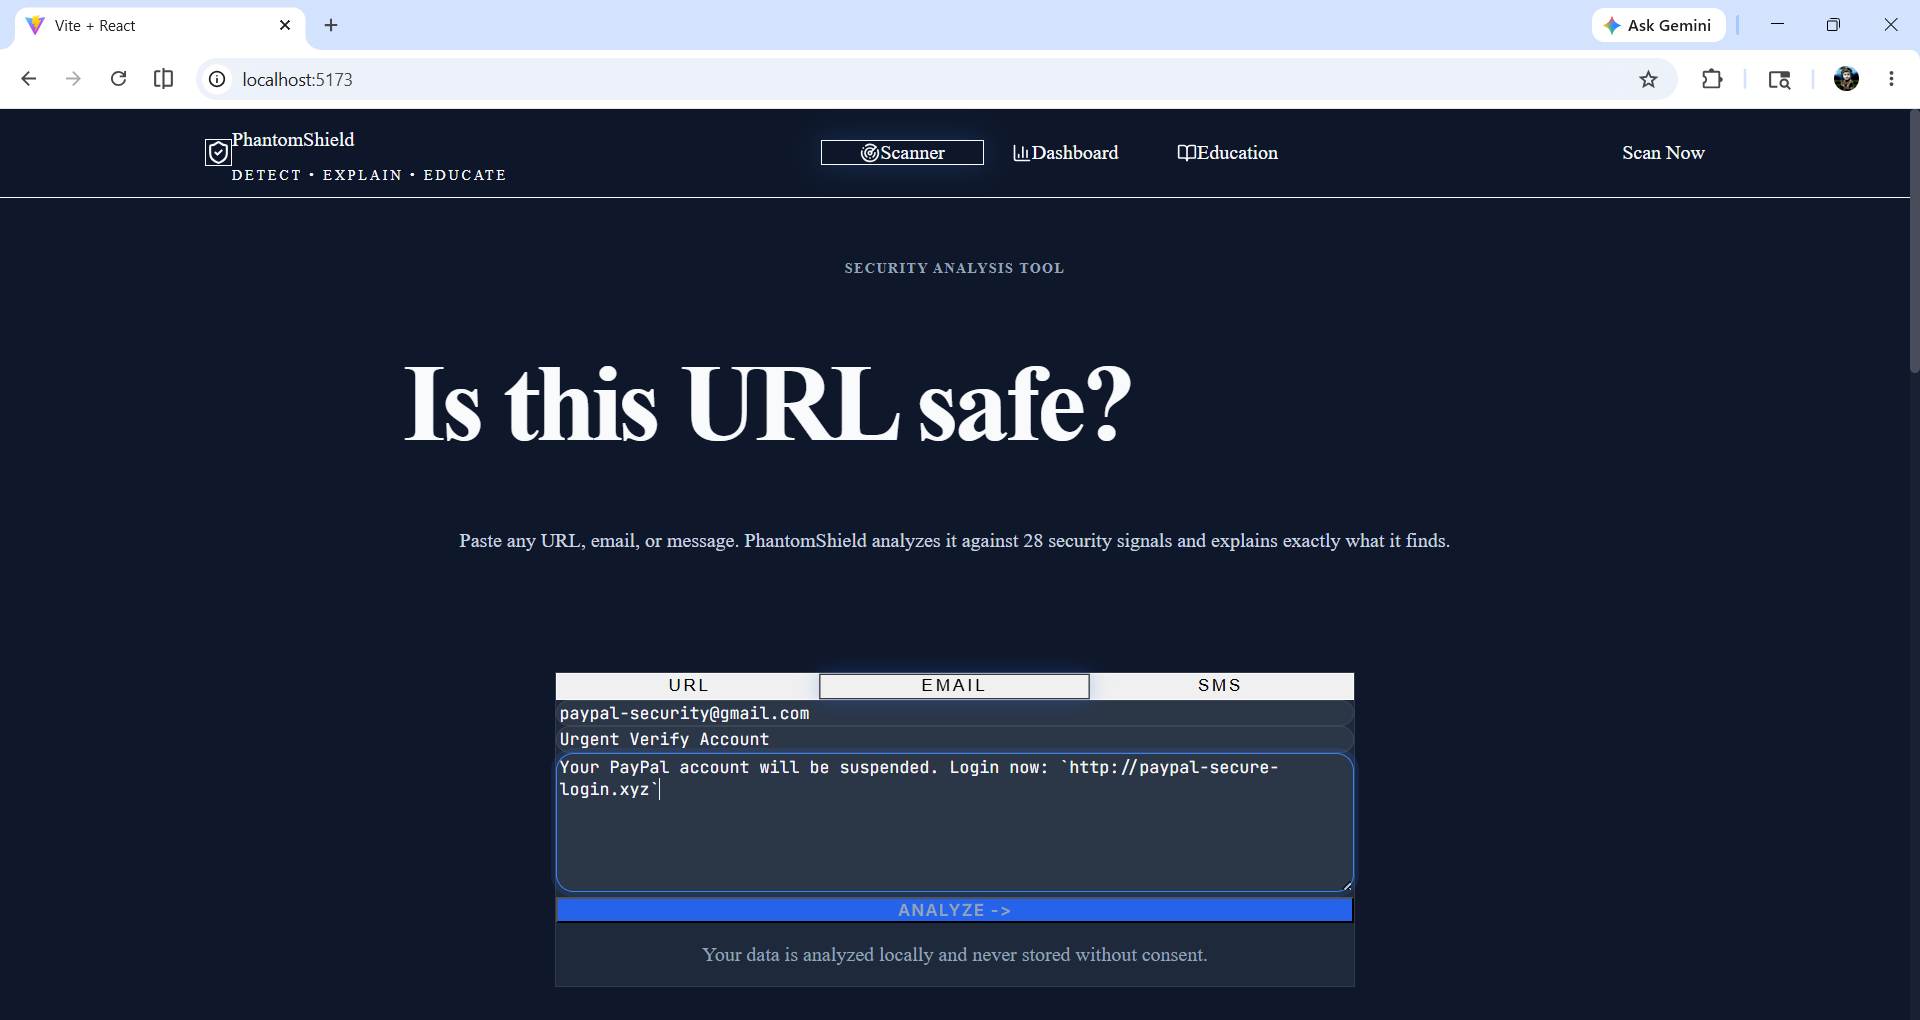
\includegraphics[width=0.98\linewidth]{screenshots/email.png}
    \caption{Email scan interface with fields for sender, subject, and message body.}
    \label{fig:email}
\end{figure}

\begin{figure}[ht]
    \centering
    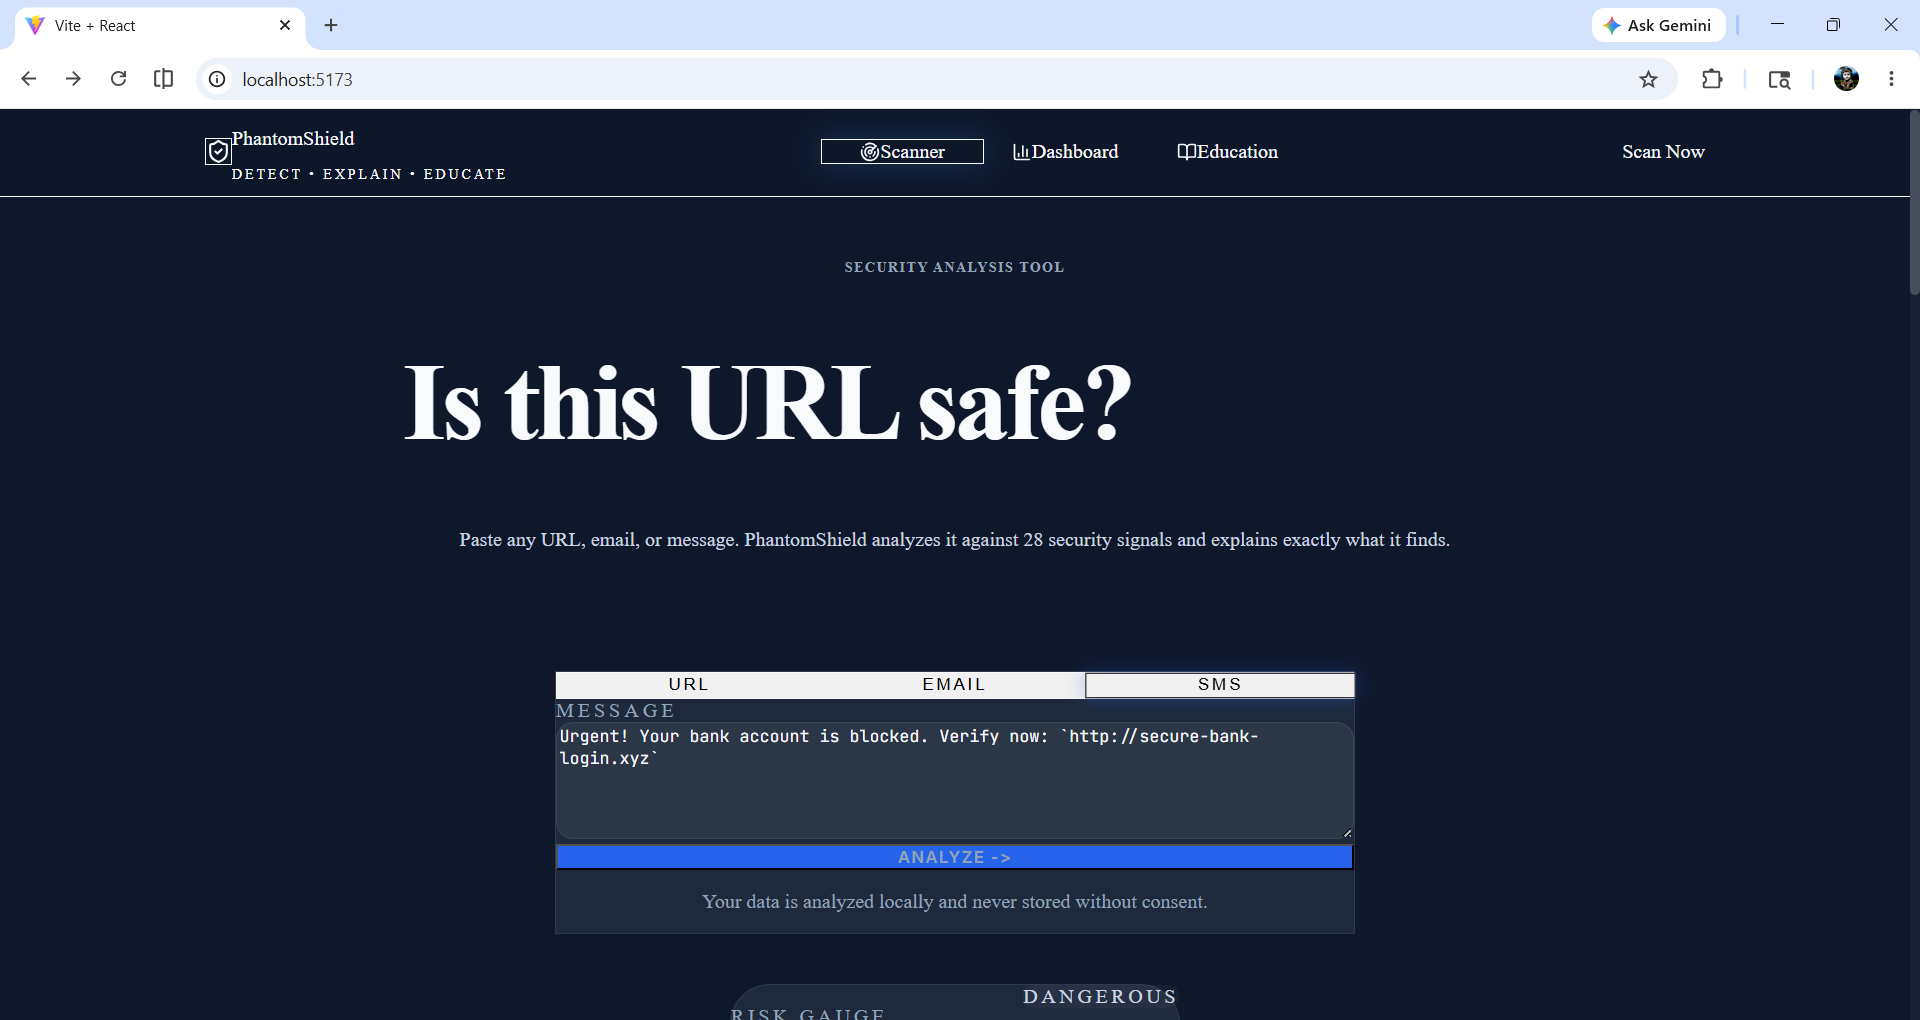
\includegraphics[width=0.98\linewidth]{screenshots/sms.png}
    \caption{SMS scan interface capturing message content for urgency-based phishing analysis.}
    \label{fig:sms}
\end{figure}

\begin{figure}[ht]
    \centering
    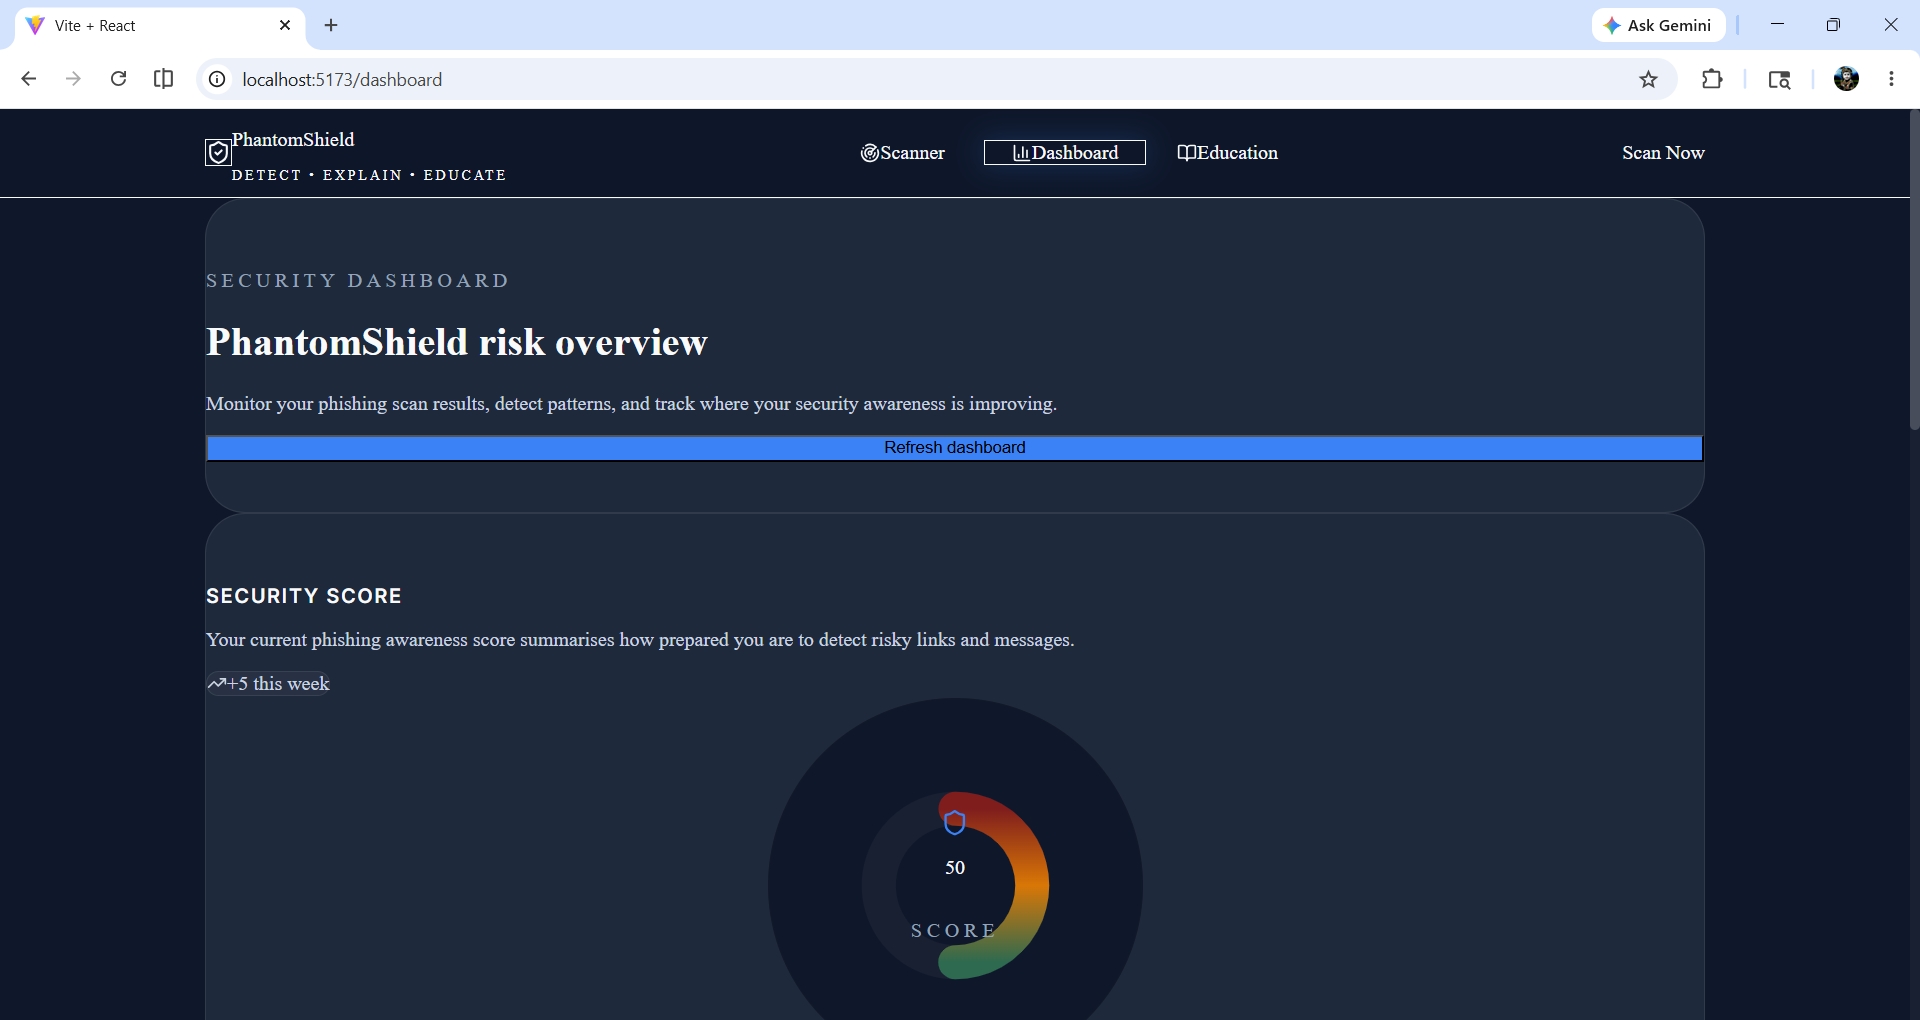
\includegraphics[width=0.98\linewidth]{screenshots/dashboard.png}
    \caption{Dashboard view showing scan history, security score, and trend metrics.}
    \label{fig:dashboard}
\end{figure}

\section{Project Plan}
Milestones and task breakdowns were followed during development. The schedule included requirement analysis, design, implementation, testing, and documentation phases.

\section{Analysis, Conclusion, and Future Work}
PhantomShield demonstrates that a hybrid phishing detection system can provide stronger protection than simple signature-based models. The combination of engineered URL features, ensemble scoring, and heuristic reasoning improves detection accuracy. The explainable frontend helps users understand why a link is dangerous.

Future work includes:
\begin{itemize}[itemsep=0pt,topsep=0pt]
    \item Adding social media and instant message scanning.
    \item Incorporating NLP-based email and SMS content analysis.
    \item Integrating external threat intelligence feeds.
    \item Enabling user feedback and adaptive model refinement.
    \item Extending support for browser extension deployment.
\end{itemize}

\section{Acknowledgement}
The author thanks the project guide, faculty, and team members for their support. Appreciation is also expressed to the authors of the reference papers and the developers of the tools used in this project.

\section*{References}
\begin{enumerate}
    \item Phishing Website Detection Using Hybrid Machine Learning Based on URL. \texttt{research paper set/Phishing Website Detection Using Hybrid_Machine.pdf}.
    \item doc\_ijraset.pdf. \texttt{research paper set/doc_ijraset.pdf}.
    \item A State-of-the-Art Review on Phishing Website Detection Techniques. \texttt{research paper set/A_State-of-the-Art_Review_on_Phishing_Website_Detection_Techniques.pdf}.
    \item A Boosting-Based Hybrid Feature Selection and Multi-Layer Stacked Ensemble Learning Model to Detect Phishing Websites. \texttt{research paper set/A_Boosting-Based_Hybrid_Feature_Selection_and_Multi-Layer_Stacked_Ensemble_Learning_Model_to_Detect_Phishing_Websites.pdf}.
    \item Evasion Attacks and Defense Mechanisms for Machine Learning-Based Web Phishing Classifiers. \texttt{research paper set/Evasion_Attacks_and_Defense_Mechanisms_for_Machine_Learning-Based_Web_Phishing_Classifiers.pdf}.
    \item A Survey on the Detection of Phishing Websites. \texttt{research paper set/Phishing_or_Not_Phishing_A_Survey_on_the_Detection_of_Phishing_Websites.pdf}.
    \item A Systematic Review Detecting Phishing Websites Using Data Mining Models. \texttt{research paper set/A_Systematic_Review_Detecting_Phishing_Websites_Using_Data_Mining_Models.pdf}.
    \item Website Phishing Attack Detection Using Innovative Meta Learning-Based Ensemble Approach. \texttt{research paper set/Website_Phishing_Attack_Detection_Using_Innovative_Meta_Learning-Based_Ensemble_Approach.pdf}.
    \item PhiKitA Phishing Kit Attacks Dataset for Phishing Websites Identification. \texttt{research paper set/PhiKitA_Phishing_Kit_Attacks_Dataset_for_Phishing_Websites_Identification.pdf}.
    \item RSTHFS A Rough Set Theory-Based Hybrid Feature Selection Method for Phishing Website Classification. \texttt{research paper set/RSTHFS_A_Rough_Set_Theory-Based_Hybrid_Feature_Selection_Method_for_Phishing_Website_Classification.pdf}.
    \item A Study on Adversarial Sample Resistance and Defense Mechanism for Multimodal Learning-Based Phishing Website Detection. \texttt{research paper set/A_Study_on_Adversarial_Sample_Resistance_and_Defense_Mechanism_for_Multimodal_Learning-Based_Phishing_Website_Detection.pdf}.
    \item Multimodal and Temporal Graph Fusion Framework for Advanced Phishing Website Detection. \texttt{research paper set/Multimodal_and_Temporal_Graph_Fusion_Framework_for_Advanced_Phishing_Website_Detection.pdf}.
    \item BGL-PhishNet Phishing Website Detection Using Hybrid Model BERT GNN and LightGBM. \texttt{research paper set/BGL-PhishNet_Phishing_Website_Detection_Using_Hybrid_Model-BERT_GNN_and_LightGBM.pdf}.
    \item Improving Phishing Website Detection using a Hybrid Two-level Framework for Feature Selection and XGBoost Tuning. \texttt{research paper set/Improving_Phishing_Website_Detection_using_a_Hybrid_Two-level_Framework_for_Feature_Selection_and_XGBoost_Tuning.pdf}.
    \item An Effective Detection Approach for Phishing URL Using ResMLP. \texttt{research paper set/An_Effective_Detection_Approach_for_Phishing_URL_Using_ResMLP.pdf}.
    \item Phishing Detection System Through Hybrid Machine Learning Based on URL. \texttt{research paper set/Phishing_Detection_System_Through_Hybrid_Machine_Learning_Based_on_URL.pdf}.
    \item ChatPhishDetector Detecting Phishing Sites Using Large Language Models. \texttt{research paper set/ChatPhishDetector_Detecting_Phishing_Sites_Using_Large_Language_Models.pdf}.
    \item Multimodal Phishing Detection on Social Networking Sites A Systematic Review. \texttt{research paper set/Multimodal_Phishing_Detection_on_Social_Networking_Sites_A_Systematic_Review.pdf}.
    \item A Survey of Intelligent Detection Designs of HTML URL Phishing Attacks. \texttt{research paper set/A_Survey_of_Intelligent_Detection_Designs_of_HTML_URL_Phishing_Attacks.pdf}.
    \item Multi-Modal Comparative Analysis on Execution of Phishing Detection Using Artificial Intelligence. \texttt{research paper set/Multi-Modal_Comparative_Analysis_on_Execution_of_Phishing_Detection_Using_Artificial_Intelligence.pdf}.
\end{enumerate}

\end{document}
